%**************************************%
%* Generated from MathBook XML source *%
%*    on 2016-08-14T13:15:40-04:00    *%
%*                                    *%
%*   http://mathbook.pugetsound.edu   *%
%*                                    *%
%**************************************%
\documentclass[10pt,]{book}
%% Load geometry package to allow page margin adjustments
\usepackage{geometry}
\geometry{letterpaper,total={5.0in,9.0in}}
%% Custom Preamble Entries, early (use latex.preamble.early)
%% Inline math delimiters, \(, \), need to be robust
%% 2016-01-31:  latexrelease.sty  supersedes  fixltx2e.sty
%% If  latexrelease.sty  exists, bugfix is in kernel
%% If not, bugfix is in  fixltx2e.sty
%% See:  https://tug.org/TUGboat/tb36-3/tb114ltnews22.pdf
%% and read "Fewer fragile commands" in distribution's  latexchanges.pdf
\IfFileExists{latexrelease.sty}{}{\usepackage{fixltx2e}}
%% Page Layout Adjustments (latex.geometry)
%% This LaTeX file may be compiled with pdflatex, xelatex, or lualatex
%% The following provides engine-specific capabilities
%% Generally, xelatex and lualatex will do better languages other than US English
%% You can pick from the conditional if you will only ever use one engine
\usepackage{ifthen}
\usepackage{ifxetex,ifluatex}
\ifthenelse{\boolean{xetex} \or \boolean{luatex}}{%
%% begin: xelatex and lualatex-specific configuration
%% fontspec package will make Latin Modern (lmodern) the default font
\ifxetex\usepackage{xltxtra}\fi
\usepackage{fontspec}
%% realscripts is the only part of xltxtra relevant to lualatex 
\ifluatex\usepackage{realscripts}\fi
%% 
%% Extensive support for other languages
\usepackage{polyglossia}
\setdefaultlanguage{english}
%% Magyar (Hungarian)
\setotherlanguage{magyar}
%% Spanish
\setotherlanguage{spanish}
%% Vietnamese
\setotherlanguage{vietnamese}
%% end: xelatex and lualatex-specific configuration
}{%
%% begin: pdflatex-specific configuration
%% translate common Unicode to their LaTeX equivalents
%% Also, fontenc with T1 makes CM-Super the default font
%% (\input{ix-utf8enc.dfu} from the "inputenx" package is possible addition (broken?)
\usepackage[T1]{fontenc}
\usepackage[utf8]{inputenc}
%% end: pdflatex-specific configuration
}
%% Monospace font: Inconsolata (zi4)
%% Sponsored by TUG: http://levien.com/type/myfonts/inconsolata.html
%% See package documentation for excellent instructions
%% One caveat, seem to need full file name to locate OTF files
%% Loads the "upquote" package as needed, so we don't have to
%% Upright quotes might come from the  textcomp  package, which we also use
%% We employ the shapely \ell to match Google Font version
%% pdflatex: "varqu" option produces best upright quotes
%% xelatex,lualatex: add StylisticSet 1 for shapely \ell
%% xelatex,lualatex: add StylisticSet 2 for plain zero
%% xelatex,lualatex: we add StylisticSet 3 for upright quotes
%% 
\ifthenelse{\boolean{xetex} \or \boolean{luatex}}{%
%% begin: xelatex and lualatex-specific monospace font
\usepackage{zi4}
\setmonofont[BoldFont=Inconsolatazi4-Bold.otf,StylisticSet={1,3}]{Inconsolatazi4-Regular.otf}
%% end: xelatex and lualatex-specific monospace font
}{%
%% begin: pdflatex-specific monospace font
\usepackage[varqu]{zi4}
%% end: pdflatex-specific monospace font
}
%% Symbols, align environment, bracket-matrix
\usepackage{amsmath}
\usepackage{amssymb}
%% allow more columns to a matrix
%% can make this even bigger by overriding with  latex.preamble.late  processing option
\setcounter{MaxMatrixCols}{30}
%%
%% Color support, xcolor package
%% Always loaded.  Used for:
%% mdframed boxes, add/delete text, author tools
\PassOptionsToPackage{usenames,dvipsnames,svgnames,table}{xcolor}
\usepackage{xcolor}
%%
%% Semantic Macros
%% To preserve meaning in a LaTeX file
%% Only defined here if required in this document
%% Used for inline definitions of terms
\newcommand{\terminology}[1]{\textbf{#1}}
%% Subdivision Numbering, Chapters, Sections, Subsections, etc
%% Subdivision numbers may be turned off at some level ("depth")
%% A section *always* has depth 1, contrary to us counting from the document root
%% The latex default is 3.  If a larger number is present here, then
%% removing this command may make some cross-references ambiguous
%% The precursor variable $numbering-maxlevel is checked for consistency in the common XSL file
\setcounter{secnumdepth}{3}
%% Environments with amsthm package
%% Theorem-like environments in "plain" style, with or without proof
\usepackage{amsthm}
\theoremstyle{plain}
%% Numbering for Theorems, Conjectures, Examples, Figures, etc
%% Controlled by  numbering.theorems.level  processing parameter
%% Always need a theorem environment to set base numbering scheme
%% even if document has no theorems (but has other environments)
\newtheorem{theorem}{Theorem}[section]
%% Only variants actually used in document appear here
%% Style is like a theorem, and for statements without proofs
%% Numbering: all theorem-like numbered consecutively
%% i.e. Corollary 4.3 follows Theorem 4.2
\newtheorem{corollary}[theorem]{Corollary}
%% Definition-like environments, normal text
%% Numbering is in sync with theorems, etc
\theoremstyle{definition}
\newtheorem{definition}[theorem]{Definition}
%% Example-like environments, normal text
%% Numbering is in sync with theorems, etc
\theoremstyle{definition}
\newtheorem{example}[theorem]{Example}
%% Miscellaneous environments, normal text
%% Numbering for inline exercises and lists is in sync with theorems, etc
\theoremstyle{definition}
\newtheorem{exercise}[theorem]{Exercise}
%% Localize LaTeX supplied names (possibly none)
\renewcommand*{\proofname}{Proof}
\renewcommand*{\chaptername}{Chapter}
%% For improved tables
\usepackage{array}
%% Some extra height on each row is desirable, especially with horizontal rules
%% Increment determined experimentally
\setlength{\extrarowheight}{0.2ex}
%% Define variable thickness horizontal rules, full and partial
%% Thicknesses are 0.03, 0.05, 0.08 in the  booktabs  package
\makeatletter
\newcommand{\hrulethin}  {\noalign{\hrule height 0.04em}}
\newcommand{\hrulemedium}{\noalign{\hrule height 0.07em}}
\newcommand{\hrulethick} {\noalign{\hrule height 0.11em}}
%% We preserve a copy of the \setlength package before other
%% packages (extpfeil) get a chance to load packages that redefine it
\let\oldsetlength\setlength
\newlength{\Oldarrayrulewidth}
\newcommand{\crulethin}[1]%
{\noalign{\global\oldsetlength{\Oldarrayrulewidth}{\arrayrulewidth}}%
\noalign{\global\oldsetlength{\arrayrulewidth}{0.04em}}\cline{#1}%
\noalign{\global\oldsetlength{\arrayrulewidth}{\Oldarrayrulewidth}}}%
\newcommand{\crulemedium}[1]%
{\noalign{\global\oldsetlength{\Oldarrayrulewidth}{\arrayrulewidth}}%
\noalign{\global\oldsetlength{\arrayrulewidth}{0.07em}}\cline{#1}%
\noalign{\global\oldsetlength{\arrayrulewidth}{\Oldarrayrulewidth}}}
\newcommand{\crulethick}[1]%
{\noalign{\global\oldsetlength{\Oldarrayrulewidth}{\arrayrulewidth}}%
\noalign{\global\oldsetlength{\arrayrulewidth}{0.11em}}\cline{#1}%
\noalign{\global\oldsetlength{\arrayrulewidth}{\Oldarrayrulewidth}}}
%% Single letter column specifiers defined via array package
\newcolumntype{A}{!{\vrule width 0.04em}}
\newcolumntype{B}{!{\vrule width 0.07em}}
\newcolumntype{C}{!{\vrule width 0.11em}}
\makeatother
%% Figures, Tables, Listings, Floats
%% The [H]ere option of the float package fixes floats in-place,
%% in deference to web usage, where floats are totally irrelevant
%% We re/define the figure, table and listing environments, if used
%%   1) New mbxfigure and/or mbxtable environments are defined with float package
%%   2) Standard LaTeX environments redefined to use new environments
%%   3) Standard LaTeX environments redefined to step theorem counter
%%   4) Counter for new environments is set to the theorem counter before caption
%% You can remove all this figure/table setup, to restore standard LaTeX behavior
%% HOWEVER, numbering of figures/tables AND theorems/examples/remarks, etc
%% WILL ALL de-synchronize with the numbering in the HTML version
%% You can remove the [H] argument of the \newfloat command, to allow flotation and 
%% preserve numbering, BUT the numbering may then appear "out-of-order"
\usepackage{float}
\usepackage[bf]{caption} % http://tex.stackexchange.com/questions/95631/defining-a-new-type-of-floating-environment 
\usepackage{newfloat}
% Figure environment setup so that it no longer floats
\SetupFloatingEnvironment{figure}{fileext=lof,placement={H},within=section,name=Figure}
% figures have the same number as theorems: http://tex.stackexchange.com/questions/16195/how-to-make-equations-figures-and-theorems-use-the-same-numbering-scheme 
\makeatletter
\let\c@figure\c@theorem
\makeatother
% Table environment setup so that it no longer floats
\SetupFloatingEnvironment{table}{fileext=lot,placement={H},within=section,name=Table}
% tables have the same number as theorems: http://tex.stackexchange.com/questions/16195/how-to-make-equations-figures-and-theorems-use-the-same-numbering-scheme 
\makeatletter
\let\c@table\c@theorem
\makeatother
%% Raster graphics inclusion, wrapped figures in paragraphs
%% \resizebox sometimes used for images in side-by-side layout
\usepackage{graphicx}
%%
%% Multiple column, column-major lists
\usepackage{multicol}
%% More flexible list management, esp. for references and exercises
%% But also for specifying labels (i.e. custom order) on nested lists
\usepackage{enumitem}
%% Lists of references in their own section, maximum depth 1
\newlist{referencelist}{description}{4}
\setlist[referencelist]{leftmargin=!,labelwidth=!,labelsep=0ex,itemsep=1.0ex,topsep=1.0ex,partopsep=0pt,parsep=0pt}
%% Lists of exercises in their own section, maximum depth 4
\newlist{exerciselist}{description}{4}
\setlist[exerciselist]{leftmargin=0pt,itemsep=1.0ex,topsep=1.0ex,partopsep=0pt,parsep=0pt}
%% Indented groups of exercises within an exercise section, maximum depth 4
\newlist{exercisegroup}{description}{4}
\setlist[exercisegroup]{leftmargin=2em,labelindent=2em,itemsep=1.0ex,topsep=1.0ex,partopsep=0pt,parsep=0pt}
%% Support for index creation
%% imakeidx package does not require extra pass (as with makeidx)
%% We set the title of the "Index" section via a keyword
%% And we provide language support for the "see" phrase
\usepackage{imakeidx}
\makeindex[title=Index, intoc=true]
\renewcommand{\seename}{see}
%% hyperref driver does not need to be specified
\usepackage{hyperref}
%% configure hyperref's  \url  to match listings' inline verbatim
\renewcommand\UrlFont{\small\ttfamily}
%% Hyperlinking active in PDFs, all links solid and blue
\hypersetup{colorlinks=true,linkcolor=blue,citecolor=blue,filecolor=blue,urlcolor=blue}
\hypersetup{pdftitle={Applied Discrete Structures}}
%% If you manually remove hyperref, leave in this next command
\providecommand\phantomsection{}
%% If tikz has been loaded, replace ampersand with \amp macro
%% extpfeil package for certain extensible arrows,
%% as also provided by MathJax extension of the same name
%% NB: this package loads mtools, which loads calc, which redefines
%%     \setlength, so it can be removed if it seems to be in the 
%%     way and your math does not use:
%%     
%%     \xtwoheadrightarrow, \xtwoheadleftarrow, \xmapsto, \xlongequal, \xtofrom
%%     
%%     we have had to be extra careful with variable thickness
%%     lines in tables, and so also load this package late
\usepackage{extpfeil}
%% Custom Preamble Entries, late (use latex.preamble.late)
%% Begin: Author-provided macros
%% (From  docinfo/macros  element)
%% Plus three from MBX for XML characters
\newcommand{\identity}{\mathrm{id}}
\newcommand{\notdivide}{{\not{\mid}}}
\newcommand{\notsubset}{\not\subset}
\newcommand{\lcm}{\operatorname{lcm}}
\newcommand{\gf}{\operatorname{GF}}
\newcommand{\inn}{\operatorname{Inn}}
\newcommand{\aut}{\operatorname{Aut}}
\newcommand{\Hom}{\operatorname{Hom}}
\newcommand{\cis}{\operatorname{cis}}
\newcommand{\chr}{\operatorname{char}}
\newcommand{\Null}{\operatorname{Null}}
\newcommand{\lt}{ < }
\newcommand{\gt}{ > }
\newcommand{\amp}{ & }
%% End: Author-provided macros
%% Title page information for book
\title{Applied Discrete Structures}
\author{Al Doerr\\
Department of Mathematical Sciences\\
University of Massachusetts Lowell\\
\href{mailto:}{\nolinkurl{}}
\and
Ken Levasseur\\
Department of Mathematical Sciences\\
University of Massachusetts Lowell\\
\href{mailto:kenneth_levasseur@uml.edu}{\nolinkurl{kenneth_levasseur@uml.edu}}
}
\date{September, 2016}
\begin{document}
\frontmatter
%% begin: half-title
\thispagestyle{empty}
{\centering
\vspace*{0.28\textheight}
{\Huge Applied Discrete Structures}\\}
\clearpage
%% end:   half-title
%% begin: adcard
\thispagestyle{empty}
\null%
\clearpage
%% end:   adcard
%% begin: title page
%% Inspired by Peter Wilson's "titleDB" in "titlepages" CTAN package
\thispagestyle{empty}
{\centering
\vspace*{0.14\textheight}
{\Huge Applied Discrete Structures}\\[3\baselineskip]
{\Large Al Doerr}\\[0.5\baselineskip]
{\Large University of Massachusetts Lowell}\\[3\baselineskip]
{\Large Ken Levasseur}\\[0.5\baselineskip]
{\Large University of Massachusetts Lowell}\\[3\baselineskip]
{\Large September, 2016}\\}
\clearpage
%% end:   title page
%% begin: copyright-page
\thispagestyle{empty}
\vspace*{\stretch{2}}
\noindent\textcopyright\ 2016\quad{}Al Doerr, Ken Levasseur\\[0.5\baselineskip]
Applied Discrete Structures by Alan Doerr and Kenneth Levasseur is licensed under a Creative Commons Attribution-NonCommercial-ShareAlike 3.0 United States License. You are free to Share: copy and redistribute the material in any medium or format; Adapt: remix, transform, and build upon the material. You may not use the material for commercial purposes.  The licensor cannot revoke these freedoms as long as you follow the license terms.
			\par
\vspace*{\stretch{1}}
\null\clearpage
%% end:   copyright-page
%% begin: acknowledgement
\chapter*{Acknowledgements}\label{acknowledgement-1}
\addcontentsline{toc}{chapter}{Acknowledgements}
I would like to thank Rob Beezer, David Farmer and other participants on the \href{https://groups.google.com/forum/?fromgroups#!forum/mathbook-xml-support}{mathbook-xml-support group} for their guidance and work on MathBook XML.  Thanks to the Pedagogy Subcommittee of the UMass Lowell Transformational Education Committee for their financial assistance in helping getting this project started.%
%% end:   acknowledgement
%% begin: preface
\chapter*{Preface}\label{preface-1}
\addcontentsline{toc}{chapter}{Preface}
This version of \emph{Applied Discrete Structures} is being developed using \emph{Mathbook XML}, A lightweight XML application for authors of scientific articles, textbooks and monographs initiated by Rob Beezer, U. of Puget Sound.  %
\par
Sage (\href{http://sagemath.org}{sagemath.org}) is a free, open source, software system for advanced mathematics.  Sage can be used either on your own computer, a local server, or on SageMathCloud (\href{https://cloud.sagemath.com}{https://cloud.sagemath.com}). %
\par\hfill\begin{tabular}{l@{}}
Ken Levasseur\\
Lowell MA
\end{tabular}\\\par
%% end:   preface
%% begin: table of contents
\setcounter{tocdepth}{1}
\renewcommand*\contentsname{Contents}
\tableofcontents
%% end:   table of contents
\mainmatter
\typeout{************************************************}
\typeout{Chapter 1 More on Sets}
\typeout{************************************************}
\chapter[More on Sets]{More on Sets}\label{chapter_4}
\typeout{************************************************}
\typeout{Introduction  }
\typeout{************************************************}

In this chapter we shall look more closely at some basic facts about sets. One question we could ask ourselves is: Can we manipulate sets similarly to the way we manipulated expressions in basic algebra, or to the way we manipulated propositions in logic? In basic algebra we are aware that \(a \cdot  (b + c) = a\cdot  b + a \cdot  c\) for all real numbers \(a\), \(b\), and \(c\). In logic we verified an analogue of this statement, namely, \(p
\land  ( q \lor  r) \Leftrightarrow  (p \land  q)\lor  (p \land  r))\), where \(p, q, \textrm{ and } r\) were arbitrary propositions. If \(A\), \(B\), and \(C\) are arbitrary sets, is \(A \cap  (B \cup  C) = (A \cap  B) \cup  (A \cap  C)\)? How do we convince ourselves of it is truth, or discover that it is false? Let us consider some approaches to this problem, look at their pros and cons, and determine their validity. Many of the ideas expressed are true, in general, in mathematics. Later in this chapter, we introduce partitions of sets and minsets.
%
\typeout{************************************************}
\typeout{Section 1.1 Methods of Proof for Sets }
\typeout{************************************************}
\section[Methods of Proof for Sets ]{Methods of Proof for Sets }\label{s-proof-methods-sets}
\typeout{************************************************}
\typeout{Introduction  }
\typeout{************************************************}
If \(A\), \(B\), and \(C\) are arbitrary sets, is it always true that \(A \cap  (B \cup  C) = (A \cap  B) \cup  (A 
\cap  C)\)?  There are a variety of ways that we could attempt to prove that this distributive law for intersection over union is indeed true We start with a common ``non-proof'' and then work toward more acceptable methods.%
\typeout{************************************************}
\typeout{Subsection 1.1.1 Examples and Counterexamples}
\typeout{************************************************}
\subsection[Examples and Counterexamples]{Examples and Counterexamples}\label{ss-examples-and-counterexamples}
We could, for example, let \(A = \{1, 2\}\), \(B = \{5, 8, 10\}\), and \(C = \{3, 2, 5\}\), and determine whether the distributive law is true for these values of \(A\), \(B\), and \(C\). In doing this we will have only determined that the distributive law is true for this one example. It does not prove the distributive law for all possible sets \(A\), \(B\), and \(C\) and hence is an invalid method of proof. However, trying a few examples has considerable merit insofar as it makes us more comfortable with the statement in question, and indeed if the statement is not true for the example, we have disproved the statement.%
\begin{definition}[Counterexample]\label{def-counterexample}
An example that disproves a statement is called a counterexample.%
\end{definition}
\begin{example}[Disproving distributivity of addition over multiplication]\label{ex-addition-over-mult}
 From basic algebra we learned that multiplication is distributive over addition. Is addition distributive over multiplication?
That is, is \(a + (b \cdot  c) = (a + b) \cdot  (a + c)\) always true? If we choose the values \(a = 3\), \(b = 4\), and \(c = 1\), we find that \(3 + (4 \cdot  1) \neq  (3 + 4)\cdot (3 + 1)\). Therefore, this set of values serves as a counterexample to a distributive law of addition over multiplication.%
\end{example}
\typeout{************************************************}
\typeout{Subsection 1.1.2 Proof Using Venn Diagrams}
\typeout{************************************************}
\subsection[Proof Using Venn Diagrams]{Proof Using Venn Diagrams}\label{ss-venn-proofs}
In this method, we illustrate both sides of the statement via a Venn diagram and determine whether both Venn diagrams give us the same ``picture,'' For example, the left side of the distributive law is developed in Figure \hyperref[distrib-venn-lhs]{\ref{distrib-venn-lhs}} and the right side in Figure \hyperref[distrib-venn-rhs]{\ref{distrib-venn-rhs}}. Note that the final results give you the same shaded area.%
\par
The advantage of this method is that it is relatively quick and mechanical. The disadvantage is that it is workable only if there are a small number of sets under consideration. In addition, it doesn't work very well in a static environment like a book or test paper.  Venn diagrams tend to work well if you have a potentially dynamic environment like a blackboard or video. 
%
\leavevmode%
\begin{figure}
\centering
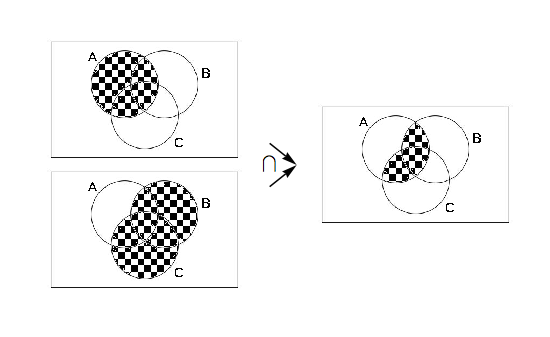
\includegraphics[width=1\linewidth]{images/distrib-venn-lhs.png}
\caption{Development of the left side of the distributive law for sets
			 \label{distrib-venn-lhs}}
\end{figure}
\leavevmode%
\begin{figure}
\centering
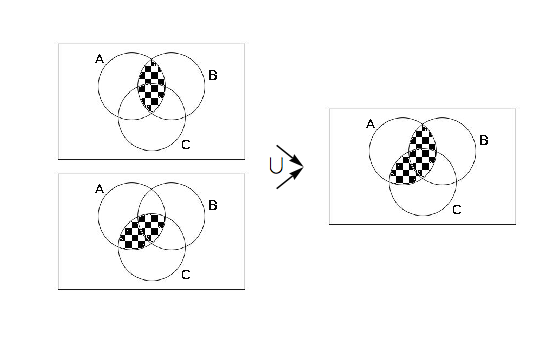
\includegraphics[width=1\linewidth]{images/distrib-venn-rhs.png}
\caption{Development of the right side of the distributive law for sets
			 \label{distrib-venn-rhs}}
\end{figure}
\typeout{************************************************}
\typeout{Subsection 1.1.3 Proof using Set-membership Tables}
\typeout{************************************************}
\subsection[Proof using Set-membership Tables]{Proof using Set-membership Tables}\label{ss-membership-table-proof}
Let \(A\) be a subset of a universal set \(U\) and let \(u\in U\). To use this method we note that exactly one of the following is true: \(u \in  A\) or \(u\notin  A\). Denote the situation where \(u \in  A\) by 1 and that where \(u \notin  A\) by 0. Working with two sets, \(A\) and \(B\), and if \(u \in  U\), there are four possible outcomes of ``where \(u\) can be.'' What are they? The set-membership table for \(A \cup  B\) is:%
\leavevmode%
\begin{table}
\centering
\begin{tabular}{ccc}
 \(A\)  & \(B\)  &\(A \cup  B\)\tabularnewline[0pt]
 0 & 0 & 0 \tabularnewline[0pt]
 0 & 1 & 1 \tabularnewline[0pt]
 1 & 0 & 1 \tabularnewline[0pt]
 1 & 1 & 1 
\end{tabular}
\caption{Membership Table for \(A \cup  B\)\label{mt-union}}
\end{table}
\par
This table illustrates that \(u\in A \cup  B\) if and only if \(a\in A\) or \(u \in  B\).%
\par
In order to prove the distributive law via a set-membership table, write out the table for each side of the set statement to be proved and note that if \(S\) and \(T\) are two columns in a table, then the set statement \(S\) is equal to the set statement \(T\) if and only if corresponding entries in each row are the same.%
\par
To prove \(A \cap  (B \cup  C) = (A \cap  B) \cup  (A \cap  C)\), first note that the statement involves three sets, \(A\), \(B\), and \(C\), So there are \(2^3= 8\) possibilities for the membership of an element in the sets.%
\leavevmode%
\begin{table}
\centering
\begin{tabular}{cccccccc}
\(A\)&\(B\)&\(C\)&\(B \cup  C\)&\(A \cap B\)&\(A \cap C\)&\(A \cap  (B \cup  C)\)&\( (A \cap  B) \cup  (A \cap  C)\)\tabularnewline[0pt]
0&0&0&0&0&0&0&0\tabularnewline[0pt]
0&0&1&1&0&0&0&0\tabularnewline[0pt]
0&1&0&1&0&0&0&0\tabularnewline[0pt]
0&1&1&1&0&0&0&0\tabularnewline[0pt]
1&0&0&0&0&0&0&0\tabularnewline[0pt]
1&0&1&1&0&1&1&1\tabularnewline[0pt]
1&1&0&1&1&0&1&1\tabularnewline[0pt]
1&1&1&1&1&1&1&1
\end{tabular}
\caption{Membership table to prove the distributive law of intersection over union\label{tab-mt-distr}}
\end{table}
\par
Since each entry in Column 7 is the same as the corresponding entry in Column 8, we have shown that \(A\cup  (B \cup  C) = (A\cap B) \cup  (A \cap C)\) for any sets \(A\), \(B\), and \(C\). The main advantage of this method is that it is mechanical. The main disadvantage is that it is reasonable to use only for a relatively small number of sets. If we are trying to prove a statement involving five sets, there are \(2^5 = 32\) rows, which would test anyone's patience doing the work by hand. %
\typeout{************************************************}
\typeout{Subsection 1.1.4 Proof Using Definitions}
\typeout{************************************************}
\subsection[Proof Using Definitions]{Proof Using Definitions}\label{ss-proofs-using-definitions-sets}
This method involves using definitions and basic concepts to prove the given statement. This procedure forces one to learn, relearn, and understand basic definitions and concepts. It helps individuals to focus their attention on the main ideas of each topic and therefore is the most useful method of proof. One does not learn a topic by memorizing or occasionally glancing at core topics, but by using them in a variety of contexts. The word proof panics most people; however, everyone can become comfortable with proofs. Do not expect to prove every statement immediately. In fact, it is not our purpose to prove every theorem or fact encountered, only those that illustrate methods and/or basic concepts. Throughout the text we will
focus in on main techniques of proofs. Let's illustrate by proving the distributive law.%
\par
 \emph{Proof Technique 1.}  State or restate the theorem so you understand what is given (the hypothesis) and what you are trying to prove (the conclusion).%
\begin{theorem}[The Distributive Law of Intersection over Union]\label{th-distr-law-i-over-u}
If \(A\), \(B\), and \(C\) are sets, then \(A\cap  (B \cup  C) = (A\cap B) \cup  (A \cap  C)\).%
\end{theorem}
\begin{proof}\hypertarget{proof-1}{}
What we can assume: \(A\), \(B\), and \(C\) are sets.%
\par
What we are to prove: : \(A\cap  (B \cup  C) = (A\cap B) \cup  (A \cap  C)\).%
\par
Commentary: What types of objects am I working with: sets? real numbers? propositions? The answer is sets: sets of elements
that can be anything you care to imagine. The universe from which we draw our elements plays no part in the proof of this theorem.%
\par
We need to show that the two sets are equal. Let's call them the left-hand set \((LHS\)) and the right-hand set (\(RHS\) ) To prove that \(LHS = RHS\)., we must prove two things: (a) \(LHS\subseteq RHS\). and (b) \(RHS\subseteq L.H.S\).%
\par
To prove part a and, similarly, part b, we must show that each element of LHS is an element of RHS.  Once we have diagnosed the problem we are ready to begin.%
\par
We must prove:
(a) \(A \cap  (B \cup  C)\subseteq (A\cap B) \cup  (A\cap C)\).%
\par

Let \(x \in  A\cap (B \cup  C)\) to show \(x\in (A\cap B) \cup  (A \cap C)\):
\begin{equation*}
\begin{split}
x \in A \cap (B \cup C) & \Rightarrow x\in A \textrm{ and } (x\in B\textrm{ or } x\in C)\\
	& \quad \textrm{def. of union and intersection}\\
	& \Rightarrow  (x \in A\textrm{ and }x\in B)\textrm{ or } (x\in A\textrm{ and }x\in C)\\
	&\quad \textrm{distributive law of logic}\\
	& \Rightarrow  (x \in A \cap B) \textrm{ or } (x \in A \cap C)\\
	&\quad \textrm{def. of intersection}\\
	& \Rightarrow  (x \in (A \cap B) \cup (A \cap C)\\
	&\quad \textrm{def. of union}
 \end{split}
\end{equation*}
We must also prove (b) \((A\cap B) \cup  (A\cap C)\subseteq A \cap  (B \cup  C)\).%
\par
\begin{equation*}
\begin{split}
x\in (A\cap B) \cup  (A \cap C)& \Rightarrow  (x\in A\cap B)\text{or } (x\in A\cap C)\\
			&\quad \textrm{ Why? } \\
			& \Rightarrow (x\in A\textrm{ and }x\in B)\textrm{ or } (x\in A\textrm{ and }x\in C)\\
			&\quad\textrm{ Why? }\\
			&\Rightarrow  x\in A \textrm{ and } (x\in B\textrm{ or }x\in C)\\
			&\quad\textrm{ Why? }\\
			&\Rightarrow x\in A\cap (B\cup C)\\
			&\quad\textrm{ Why? } \square
\end{split}
 \end{equation*}%
\end{proof}
\par
\emph{Proof Technique 2}%
\par
\leavevmode%
\begin{enumerate}[label=\arabic*]
\item\hypertarget{li-1}{}To prove that \(A\subseteq B\), we must show that if \(x \in  A\), then \(x \in  B\).%
\item\hypertarget{li-2}{}To prove that \(A = B\), we must show:%
\par
%
\begin{enumerate}[label=\alph*]
\item\hypertarget{li-3}{} \(A\subseteq B\) and%
\item\hypertarget{li-4}{} \(B \subseteq A\).%
\end{enumerate}
%
\end{enumerate}
%
\par
To further illustrate the Proof-by-Definition technique, let's prove the following theorem.%
\begin{theorem}[Another Proof using Definitions]\label{th-set-proof-example2}
Let \(A\), \(B\), and \(C\) be sets, then \(A \times  (B \cap  C) = (A \times  B) \cap  (A \times  C)\).%
\end{theorem}
\begin{proof}\hypertarget{proof-2}{}
Commentary; We again ask ourselves: What are we trying to prove? What types of objects are we dealing with? We realize that we wish to prove two facts: (a) \(LHS\subseteq RHS\). and (b) \(RHS\subseteq LHS\).%
\par
To prove part a, and similarly part b, we'll begin the same way. Let  \(\_\_\_ \in  LHS\) to show \(\_\_\_ \in  RHS\). What should \(\_\_\_\) be?  What does a typical object in the \(LHS\) look like?%
\par
Now, on to the actual proof.%
\par
(a) \(A\times (B\cap  C)\subseteq (A\times B)\cap (A\times C)\).%
\par
Let \((x, y) \in  A\times (B\cap C)\) to prove\((x, y) \in  (A\times B)\cap (A\times C)\):
\begin{equation*}
\begin{split}
(x, y) \in A\times (B\cap C) &\Rightarrow x \in  A \textrm{ and } y \in  (B\cap  C)\\
	&\quad \textrm{ Why? }\\
	&\Rightarrow x \in  A \textrm{ and }(y \in  B\textrm{ and } y \in  C)\\
	&\textrm{ Why? }\\
	&\Rightarrow (x \in  A \textrm{ and } y \in  B) \textrm{ and } (x \in  A \textrm{ and } y \in C)\\
	&\quad \textrm{ Why? }\\
	  &\Rightarrow  (x, y) \in  (A\times B) \textrm{ and } (x, y) \in  (A \times C)\\
	  &\quad \textrm{ Why? }\\
	   &\Rightarrow (x, y) \in  (A\times  B) \cap (A\times C)\\
	   &\quad \textrm{ Why? }
 \end{split}
 \end{equation*}
%
\par
(b) \((A\times  B)\cap (A\times C)\subseteq A\times ( B\cap C)\):

Let \((x, y) \in  (A\times  B) \cap  (A\times C)\) to prove \((x, y) \in  A \cap  ( B\times C)\):
\begin{equation*}
\begin{split}
(x, y) \in  (A\times  B)\cap (A\times C) &\Rightarrow (x, y) \in  A\times  B\textrm{ and } (x, y) \in  A\times C\\
	&\quad \textrm{ Why? }\\
	&\Rightarrow (x \in  A \textrm{ and } y \in  B) \textrm{ and } (x \in  A \textrm{ and } y \in  C)\\
	&\quad \textrm{ Why? }\\
  &\Rightarrow  x \in  A \textrm{ and } (y \in  B\textrm{ and } y \in  C)\\
  &\quad \textrm{ Why? }\\
  &\Rightarrow  x \in  A\textrm{ and } y \in  (B\cap  C)\\
  &\quad \textrm{ Why? }\\
   &\Rightarrow (x, y) \in  A \times (B\cap  C)\\
   &\quad \textrm{ Why? }  \square
 \end{split}
 \end{equation*}
%
\end{proof}
\typeout{************************************************}
\typeout{Exercises 1.1.5 Exercises for Section 4.1}
\typeout{************************************************}
\subsection[Exercises for Section 4.1]{Exercises for Section 4.1}\label{exercises-1}
\hypertarget{exercisegroup-1}{}\typeout{************************************************}
\typeout{Introduction  }
\typeout{************************************************}
A Exercises%
\begin{exercisegroup}
\item[1.]\hypertarget{exercise-4-1-1}{} Prove the following:%
\par
\leavevmode%
\begin{enumerate}[label=\alph*]
\item\hypertarget{li-5}{}Let \(A\), \(B\), and \(C\) be sets. If \(A\subseteq B\) and \(B\subseteq C\), then \(A\subseteq C\).%
\item\hypertarget{li-6}{}Let \(A\) and \(B\) be sets. Then \(A - B= A\cap B^c\) .%
\item\hypertarget{li-7}{}Let \(A,B, \textrm{ and } C\) be sets. If (\(A\subseteq B\) and\(A\subseteq C\)) then \(A\subseteq B\cap C\).%
\item\hypertarget{li-8}{}Let \(A \textrm{ and } B\) be sets. \(A\subseteq B\) If and only if \(B^c\subseteq A^c\) .%
\item\hypertarget{li-9}{}Let \(A,B, \textrm{ and } C\) be sets. If \(A\subseteq B\) then \(A\times C \subseteq B\times C\).%
\end{enumerate}
%
\par\smallskip
\par\smallskip
\noindent\textbf{Answer.}\hypertarget{answer-1}{}\quad
\leavevmode%
\begin{enumerate}[label=\alph*]
\item\hypertarget{li-10}{} Assume that \(x\in A\) (condition of the conditional conclusion \(A \subseteq  C\)). Since \(A \subseteq  B\), \(x\in B\) by the definition of \(\subseteq\). \(B\subseteq C\) and \(x\in B\) implies that \(x\in C\). Therefore, if \(x\in A\), then \(x\in C\). \(\square\) %
\item\hypertarget{li-11}{} (Proof that \(A -B \subseteq A\cap B^c\)) Let \(x\) be in \(A - B\). Therefore, x is in \(A\), but it is not in B; that is,\(\text{  }x \in  A\) and      \(x \in  B^c \Rightarrow x\in A\cap B^c\). \(\square\)%
\item\hypertarget{li-12}{}\((\Rightarrow )\)Assume that \(A \subseteq  B\) and \(A \subseteq  C\). Let \(x\in A\). By the two premises,\(x\in B\) and \(x\in C\). Therefore, by the      definition of intersection, \(x\in B\cap C\). \(\square\)%
\item\hypertarget{li-13}{} \((\Rightarrow )\)(Indirect) Assume that \(A\subseteq C\) and \(B^c\) is not a subset of \(A^c\) . Therefore, there exists \(x\in B^c\) that does not  belong to \(A^c\). \(x \notin  A^c \Rightarrow  x \in  A\). Therefore, \(x\in A\) and \(x\notin B\), a contradiction to the assumption that \(A\subseteq B\). \(\square\)%
\end{enumerate}
%
\item[2.]\hypertarget{exercise-2}{}Write the converse of parts (a), (c), and (e) of Exercise 1 and prove or disprove them.%
\par\smallskip
\item[3.]\hypertarget{exercise-3}{}  Disprove the following, assuming \(A, B, \textrm{ and } C\) are sets:%
\par
\leavevmode%
\begin{enumerate}[label=\alph*]
\item\hypertarget{li-14}{}\(A - B = B - A\).%
\item\hypertarget{li-15}{}\(A\times B = B\times A\).%
\item\hypertarget{li-16}{}\(A \cap   B = A  \cap   C\) implies \(B = C\).%
\end{enumerate}
%
\par\smallskip
\par\smallskip
\noindent\textbf{Answer.}\hypertarget{answer-2}{}\quad
\leavevmode%
\begin{enumerate}[label=\alph*]
\item\hypertarget{li-17}{} If \(A = \mathbb{Z}\) and \(B=\emptyset\), \(A - B = \pmb{\mathbb{Z}}\), while \(B - A = \emptyset\).%
\item\hypertarget{li-18}{} If \(A=\{0\}\) and \(B = \{1\}\), \((0,1) \in  A \times  B\), but \((0, 1)\) is not in \(B\times A\).%
\item\hypertarget{li-19}{}Let \(A = \emptyset\), \(B = \{0\}\), and \(C = \{1\}\). %
\end{enumerate}
%
\item[4.]\hypertarget{exercise-4}{}  Let \(A, B, \textrm{ and } C\) be sets. Write the following in ``if . . . then . . .'' language and prove:%
\par
\leavevmode%
\begin{enumerate}[label=\alph*]
\item\hypertarget{li-20}{}\(x \in  B\) is a sufficient condition for \(x \in  A \cup B\).%
\item\hypertarget{li-21}{}\(A \cap B\cap C = \emptyset\) is a necessary condition for \(A \cap  B =\emptyset\).%
\item\hypertarget{li-22}{}\(A \cup  B = B\) is a necessary and sufficient condition for \(A\subseteq  B\).%
\end{enumerate}
%
\par\smallskip
\end{exercisegroup}
\par\smallskip\noindent
\hypertarget{exercisegroup-2}{}\typeout{************************************************}
\typeout{Introduction  }
\typeout{************************************************}
B Exercises%
\begin{exercisegroup}
\item[5.]\hypertarget{ex-generalized_distrib}{}Prove by induction that if \(A\), \(B_1\) \(B_2\) , . . . , \(B_n\), are sets, \(n\geq 2\), then 
\(A\cap ( B_1 \cup  B_2\cup  \dots  \cup  B_n) = (A \cap B_1) \cup  (A \cap B_2 ) \cup  \dots \cup  (A\cap B_n)\).%
\par\smallskip
\par\smallskip
\noindent\textbf{Solution.}\hypertarget{solution-1}{}\quad
 Proof: Let \(p(n)\) be

\begin{equation*}A\cap (B_1\cup B_2\cup \cdots \cup B_n)=(A\cap B_1)\cup (A\cap B_2)\cup \cdots \cup (A\cap B_n)\end{equation*}%
\par
Basis: We must show that \(p(2) : A \cap  (B_1 \cup B_2 )=(A\cap B_1) \cup (A\cap B_2)\) is true.
 This was done by several methods in section 4.1.%
\par
Induction: Assume for some \(n\geq 2\) that \(p(n)\) is true. Then
 \begin{equation*}
 \begin{split}
 A\cap (B_1\cup B_2\cup \cdots \cup B_{n+1})&=A\cap ((B_1\cup B_2\cup \cdots \cup B_n)\cup B_{n+1})\\
	&=(A \cap (B_1\cup B_2\cup \cdots \cup B_n))\cup (A\cap B_{n+1}) \quad \textrm{by } p(2)\\
	&=((A\cap B_1)\cup \cdots \cup (A\cap B_n))\cup (A\cap B_{n+1})\quad \textrm{by the induction hypothesis}\\
	&=(A\cap B_1)\cup \cdots \cup (A\cap B_n)\cup (A\cap B_{n+1})\quad \square\\
 \end{split}
 \end{equation*} 
%
\end{exercisegroup}
\par\smallskip\noindent
\typeout{************************************************}
\typeout{Section 1.2 Laws of Set Theory}
\typeout{************************************************}
\section[Laws of Set Theory]{Laws of Set Theory}\label{s-laws-of-set-theory}
\typeout{************************************************}
\typeout{Subsection 1.2.1 Tables of Laws}
\typeout{************************************************}
\subsection[Tables of Laws]{Tables of Laws}\label{subsection-5}
The following basic set laws can be derived using either the Basic Definition or the Set-Membership approach and can be illustrated by Venn diagrams.%
\leavevmode%
\begin{table}
\centering
\begin{tabular}{ccc}
&&\tabularnewline[0pt]
 &Commutative Laws& \tabularnewline[0pt]
(1) \(A \cup B = B \cup  A\)& &(1') \(A \cap B = B\cap A\) 
\tabularnewline\hrulethin
&Associative Laws&\tabularnewline[0pt]
(2) \(A \cup  (B \cup  C)= (A\cup B)\cup C\) &&(2') \(A \cap  (B \cap  C) = (A \cap  B) \cap  C \)\tabularnewline\hrulethin
&Distributive Laws&\tabularnewline[0pt]
(3) \(A\cap (B \cup  C)=(A\cap B )\cup (A\cap  C)\) &&(3') \(A \cup (B \cap C) = (A \cup B ) \cap (A\cup C)\)\tabularnewline\hrulethin
&Identity Laws&\tabularnewline[0pt]
(4) \(A \cup  \emptyset  = \emptyset  \cup  A = A\).&&(4') \(A \cap  U = U \cap  A = A\)
\tabularnewline\hrulethin
&Complement Laws&\tabularnewline[0pt]
(5) \(A\cup A^c= U\)&&(5') \(A\cap A^c= \emptyset\)\tabularnewline\hrulethin
&Idempotent Laws&\tabularnewline[0pt]
(6) \(A \cup  A = A\)&& (6') \(A\cap  A = A\)\tabularnewline\hrulethin
&Null Laws&\tabularnewline[0pt]
(7) \(A \cup  U = U\)&&(7') \(A \cap  \emptyset  =\emptyset\)\tabularnewline\hrulethin
&Absorption Laws&\tabularnewline[0pt]
(8) \(A \cup  (A\cap  B) = A\)&&(8') \(A\cap (A \cup  B) = A\)\tabularnewline\hrulethin
&DeMorgan's Laws&\tabularnewline[0pt]
(9) \((A \cup  B)^c= A^c\cap  B^c\)&& (9') \((A\cap  B)^c = A^c \cup  B^c\)\tabularnewline\hrulethin
&Involution Law&\tabularnewline[0pt]
&(10) \((A^c)^c= A\)&\tabularnewline\hrulethin
\end{tabular}
\caption{Basic Laws of Set Theory\label{table-set-laws}}
\end{table}
\par
It is quite clear that most of these laws resemble or, in fact, are analogues of laws in basic algebra and the algebra of propositions.%
\typeout{************************************************}
\typeout{Subsection 1.2.2 Proof Using Previously Proven Theorems}
\typeout{************************************************}
\subsection[Proof Using Previously Proven Theorems]{Proof Using Previously Proven Theorems}\label{ss-proof-with-theorems}
Once a few basic laws or theorems have been established, we frequently use them to prove additional theorems. This method of proof is usually more efficient than that of proof by Definition. To illustrate, let us prove the following Corollary to the Distributive Law.   The term "corollary" is used for theorems that can be proven with relative ease from previously proven theorems.
%
\begin{corollary}[A Corollary to the Distributive Law of Sets]\label{th-corrollary-to-distr}
Let A and B be sets. Then \((A\cap  B) \cup  (A\cap  B^c) = A\).%
\end{corollary}
\begin{proof}\hypertarget{proof-3}{}
\begin{equation*}
\begin{split}
((A\cap  B) \cup  (A\cap  B^c) & = A \cap (B \cup B^c)\\
		 & \quad Why?\\
		& = A \cap U\\ 
		&\quad  Why?\\
		& = A\\
		&\quad Why? 
\end{split}
\end{equation*}%
\end{proof}
\typeout{************************************************}
\typeout{Subsection 1.2.3 Proof Using the Indirect Method/Contradiction}
\typeout{************************************************}
\subsection[Proof Using the Indirect Method/Contradiction]{Proof Using the Indirect Method/Contradiction}\label{ss-proof-sets-contradiction}
The procedure one most frequently uses to prove a theorem in mathematics is the Direct Method, as illustrated in Theorems 4.1.1 and 4.1.2. Occasionally there are situations where this method is not applicable. Consider the following:%
\begin{theorem}[An Indirect Proof in Set Theory]\label{theorem-example-sets-contradiction}
Let \(A, B, C\) be sets. If \(A\subseteq B\) and \(B\cap C = \emptyset\), then \(A\cap C = \emptyset\).%
\end{theorem}
\begin{proof}\hypertarget{proof-4}{}
Commentary: The usual and first approach would be to assume \(A\subseteq B\) and \(B\cap C = \emptyset\) is true and to attempt to prove \(A\cap C = \emptyset\) is true. To do this you would need to show that nothing is contained in the set \(A \cap  C\). Think about how you would show that something doesn't exist. It is very difficult to do directly.%
\par
The Indirect Method is much easier: If we assume the conclusion is false and we obtain a contradiction ---  then the theorem must be true. This approach is on sound logical footing since it is exactly the same method of indirect proof that we discussed in Chapter 8.%
\par
Assume \(A\subseteq B\) and \(B\cap C = \emptyset\), and \(A\cap C \neq  \emptyset\). To prove that this cannot
occur, let \(x\in A \cap C\).%
\par
\begin{equation*}
\begin{split}
x \in A \cap C & \Rightarrow x \in A \textrm{ and } x \in  C\\
	& \Rightarrow x \in B \textrm{ and } x \in  C\\
	& \Rightarrow x \in  B \cap C
\end{split}
\end{equation*}%
\par
But this contradicts the second premise.  Hence, the theorem is proven. \(\blacksquare \) %
\end{proof}
\typeout{************************************************}
\typeout{Exercises 1.2.4 Exercises for Section 4.2"}
\typeout{************************************************}
\subsection[Exercises for Section 4.2"]{Exercises for Section 4.2"}\label{exer-4-2}
\typeout{************************************************}
\typeout{Introduction  }
\typeout{************************************************}
In the exercises that follow it is most important that you outline the logical procedures or methods you use.%
\hypertarget{exercisegroup-3}{}\typeout{************************************************}
\typeout{Introduction  }
\typeout{************************************************}
A Exercises%
\begin{exercisegroup}
\item[1.]\hypertarget{exercise-6}{}\leavevmode%
\begin{enumerate}[label=\alph*]
\item\hypertarget{li-23}{}Prove the associative law for intersection (Law 2') with a Venn diagram.%
\item\hypertarget{li-24}{}Prove DeMorgan's Law (Law 9) with a membership table.%
\item\hypertarget{li-25}{}Prove the Idempotent Law (Law 6) using basic definitions.%
\end{enumerate}
%
\par\smallskip
\par\smallskip
\noindent\textbf{Answer.}\hypertarget{answer-3}{}\quad
\leavevmode%
\begin{enumerate}[label=\alph*]
\item\hypertarget{li-26}{}%
\item\hypertarget{li-27}{}
 \[\begin{array}{ccccccc}
 A & B &A^c & B^c & A\cup B & (A\cup B)^c &A^c\cap B^c \\
 \hline
 0 & 0 &1 &  1 &  0 &  1 &  1 \\
 0 & 1 &1 &  0 &  1 &  0 &  0 \\
 1 & 0 & 0 &  1 &  1 &  0 &  0 \\
 1 & 1 & 0 &  0 &  1 &  0 &  0 \\
\end{array}\]
The last two columns are the same so the two sets must be equal.%
\item\hypertarget{li-28}{} (i) \(x\in A\cup A \Rightarrow  (x\in A) \lor (x\in A)\) by the definition of \(\cap\).
    \(\Rightarrow x\in A\) by the idempotent law of logic.
 Therefore, \(A\cup A\subseteq A\). %

(ii) \(x\in A\Rightarrow (x\in A) \lor (x\in A)\) by conjunctive addition
           \(\Rightarrow  x\in A\cup A\).
Therefore, \(A \subseteq A\cup A\) and so we have \(A\cup A=A\). \(\square\)\end{enumerate}
%
\item[2.]\hypertarget{exercise-7}{}\leavevmode%
\begin{enumerate}[label=\alph*]
\item\hypertarget{li-29}{}Prove the Absorption Law (Law 8') with a Venn diagram.%
\item\hypertarget{li-30}{}Prove the Identity Law (Law 4) with a membership table.%
\item\hypertarget{li-31}{}Prove the Involution Law (Law 10) using basic definitions.%
\end{enumerate}
%
\par\smallskip
\item[3.]\hypertarget{exercise-8}{}Prove the following using the set theory laws, as well as any other theorems proved so far.%
\par
\leavevmode%
\begin{enumerate}[label=\alph*]
\item\hypertarget{li-32}{}  \(A \cup  (B - A) = A \cup  B\)%
\item\hypertarget{li-33}{}  \(A - B = B^c - A ^c\)%
\item\hypertarget{li-34}{}  \(A\subseteq B, A\cap C \neq \emptyset  \Rightarrow  B\cap C \neq \emptyset\)%
\item\hypertarget{li-35}{}  \(A\cap (B - C) = (A\cap B) - (A\cap C)\).%
\item\hypertarget{li-36}{}  \(A - (B \cup  C) = (A - B)\cap (A - C)\)%
\end{enumerate}
%
\par\smallskip
\par\smallskip
\noindent\textbf{Answer.}\hypertarget{answer-4}{}\quad
 For all parts of this exercise, a reason should be supplied for each step. 
We have supplied reasons only for part a and left them out of the other parts to give you further practice.%
\par
\leavevmode%
\begin{enumerate}[label=\alph*]
\item\hypertarget{li-37}{}\begin{equation*}
\begin{split}
A \cup (B-A)&=A\cup (B \cap A^c) \textrm{  by Exercise 1 of Section 4.1}\\
            & =(A\cup B)\cap (A\cup A^c) \textrm{  by the distributive law}\\
            &=(A\cup B)\cap U \textrm{  by the null law}\\
              &=(A\cup B) \textrm{  by the identity law }  \square
\end{split}
	\end{equation*}%
\item\hypertarget{li-38}{}\begin{equation*}
\begin{split}
A - B & = A \cap B ^c\\
       &  =B^c\cap A\\
       &=B^c\cap (A^c)^c\\
       &=B^c-A^c\\
	\end{split}
	\end{equation*}%
\item\hypertarget{li-39}{}Select any element, \(x \in A\cap C\). One such element exists since \(A\cap C\) is not empty.
\begin{equation*}
\begin{split}
 x\in A\cap C\  &\Rightarrow x\in A \land x\in C \\
          & \Rightarrow x\in B \land x\in C \\
          & \Rightarrow x\in B\cap C \\
          & \Rightarrow B\cap C \neq \emptyset \quad \square \\
   \end{split}
	\end{equation*}%
\item\hypertarget{li-40}{}\begin{equation*}
\begin{split}
A\cap (B-C) &=A\cap (B\cap C^c) \\
				& = (A\cap B\cap A^c)\cup (A\cap B\cap C^c) \\
              & =(A\cap B)\cap (A^c\cup C^c) \\
              & =(A\cap B)\cap (A\cup C)^c \\
              & =(A-B)\cap (A-C) \quad \square\\
   \end{split}
	\end{equation*}%
\item\hypertarget{li-41}{}\begin{equation*}
\begin{split}
A-(B\cup C)& = A\cap (B\cup C)^c\\
              & =A\cap (B^c\cap C^c)\\
              & =(A\cap B^c)\cap (A\cap C^c)\\
              & =(A-B)\cap (A-C)  \quad \square\\
   \end{split}
	\end{equation*}%
\end{enumerate}
%
\item[4.]\hypertarget{exercise-9}{} Use previously proven theorems to prove the following.%
\par
\leavevmode%
\begin{enumerate}[label=\alph*]
\item\hypertarget{li-42}{}  \(A \cap (B\cap C)^c= (A\cap B^c)\cup (A\cap C^{c })\)%
\item\hypertarget{li-43}{}  \(A \cap (B\cap (A\cap B)^c)= \emptyset\)%
\item\hypertarget{li-44}{}  \((A\cap B) \cup  B^c = A \cup  B^c\)%
\item\hypertarget{li-45}{}  \(A \cup  (B - C) = (A \cup  B) - (C - A)\).%
\end{enumerate}
%
\par\smallskip
\item[5.]\hypertarget{exercise-10}{}(Hierarchy of Set Operations)\space\space{}The rules that determine the order of evaluation in a set expression that involves more than one operation are similar to the rules for logic. In the absence of parentheses, complementations are done first, intersections second, and unions third. Parentheses are used to override this order. If the same operation appears two or more consecutive times, evaluate from left to right. In what order are the
following expressions performed?%
\par
\leavevmode%
\begin{multicols}{2}
\begin{enumerate}[label=\alph*]
\item\hypertarget{li-46}{}\(A \cup  B^c\cap C\). %
\item\hypertarget{li-47}{}\(A\cap B \cup  C\cap B\). %
\item\hypertarget{li-48}{}\(A \cup  B \cup  C^c\) %
\end{enumerate}
\end{multicols}
%
\par\smallskip
\par\smallskip
\noindent\textbf{Answer.}\hypertarget{answer-5}{}\quad
\leavevmode%
\begin{multicols}{3}
\begin{enumerate}[label=\alph*]
\item\hypertarget{li-49}{} \(A\cup ((B^c)\cap C)\) %
\item\hypertarget{li-50}{} \((A\cap B)\cup (C\cap B)\) %
\item\hypertarget{li-51}{} \((A\cup B)\cup (C^c)\)%
\end{enumerate}
\end{multicols}
%
\end{exercisegroup}
\par\smallskip\noindent
\hypertarget{exercisegroup-4}{}\typeout{************************************************}
\typeout{Introduction  }
\typeout{************************************************}
C Exercise%
\begin{exercisegroup}
\item[6.]\hypertarget{exercise-11}{} There are several ways that we can use to format the proofs in this chapter. One that should be familiar to you from Chapter 3 is illustrated with the following alternate proof of part (a) in \hyperref[th-distr-law-i-over-u]{Theorem~\ref{th-distr-law-i-over-u}}:%
\leavevmode%
\begin{table}
\centering
\begin{tabular}{ccc}
(1) &\(x \in  A \cap  (B \cup  C)\)  & Premise\tabularnewline[0pt]
(2) &\((x \in  A) \land  (x \in  B \cup  C)\) & (1), definition of intersection \tabularnewline[0pt]
(3)&  (\(x \in  A) \land ((x \in  B) \lor  (x \in  C))\) &(2), definition of union  \tabularnewline[0pt]
(4)& \((x \in A)\land (x\in  B)\lor  (x \in A)\land (x\in  C)\) & (3), distribute \(\land\) over \(\lor\) \tabularnewline[0pt]
(5)& \((x \in  A\cap B) \lor (x \in  A \cap C)\) & (4), definition of intersection \tabularnewline[0pt]
(6)&  \(x \in  (A \cap B) \cup  (A \cap C)\) & (5), definition of union \(\blacksquare\) 
\end{tabular}
\caption{An alternate format for the proof of \hyperref[th-distr-law-i-over-u]{Theorem~\ref{th-distr-law-i-over-u}}\label{tt-conditional-proof}}
\end{table}
\par
Prove part (b) of \hyperref[th-set-proof-example2]{Theorem~\ref{th-set-proof-example2}} and \hyperref[theorem-example-sets-contradiction]{Theorem~\ref{theorem-example-sets-contradiction}} using this format.%
\par\smallskip
\end{exercisegroup}
\par\smallskip\noindent
\typeout{************************************************}
\typeout{Section 1.3 Minsets}
\typeout{************************************************}
\section[Minsets]{Minsets}\label{s-minsets}
Let \(B_1\) and \(B_2\) be subsets of a set \(A\). Notice that the Venn diagram of \hyperref[fig-minsets-2]{Figure~\ref{fig-minsets-2}} is naturally partitioned into the subsets \(A_1\), \(A_2\), \(A_3\), and \(A_4\). Further we observe that \(A_1\), \(A_2\), \(A_3\), and \(A_4\) can be described in terms of \(B_1\) and \(B_2\) as follows:%
\leavevmode%
\begin{figure}
\centering
\IfFileExists{images/minsets-2.pdf}%
{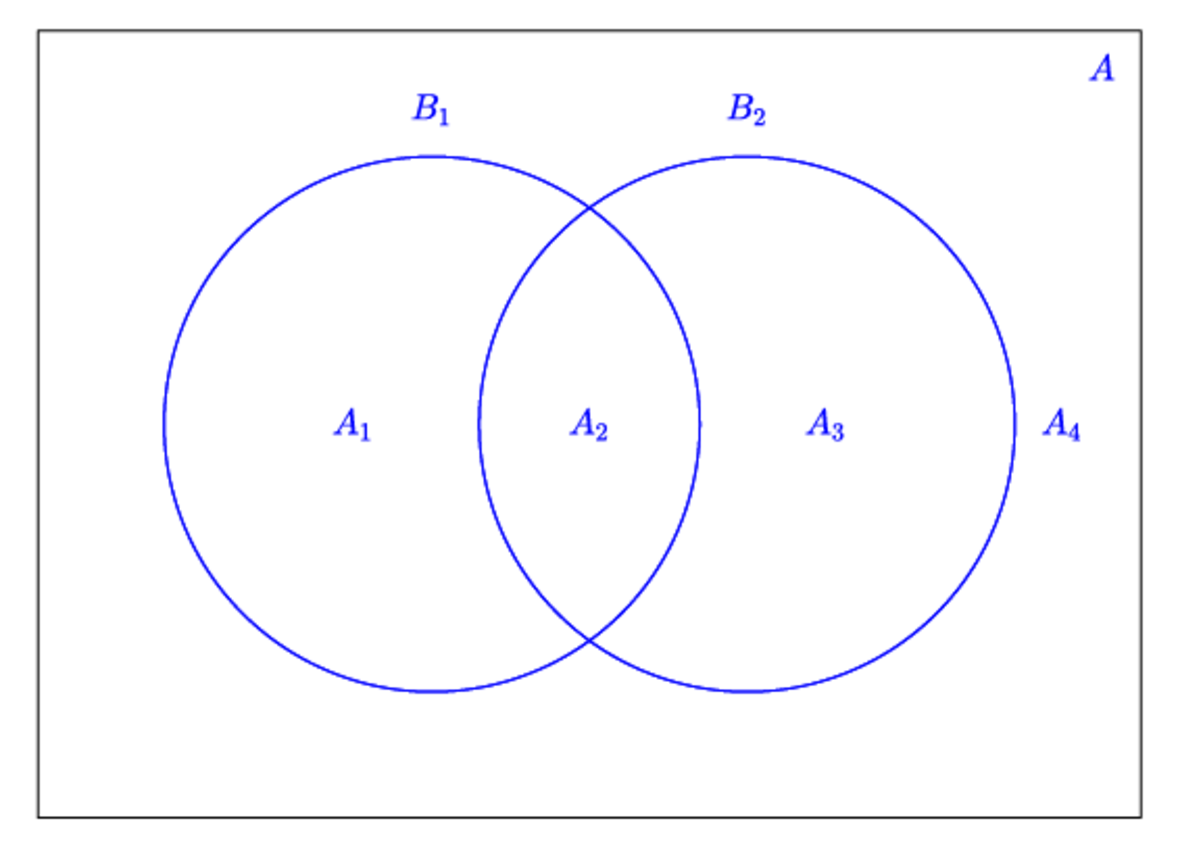
\includegraphics[width=1\linewidth]{images/minsets-2.pdf}}%
{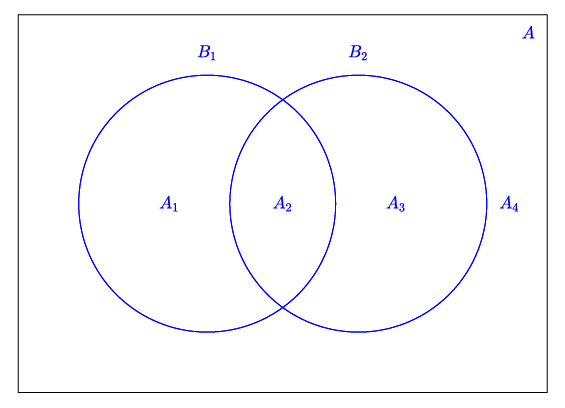
\includegraphics[width=1\linewidth]{images/minsets-2.png}}
\caption{Venn Diagram of Minsets\label{fig-minsets-2}}
\end{figure}
\leavevmode%
\begin{table}
\centering
\begin{tabular}{c}
\(A_1=B_1\cup B_2^c\)\tabularnewline[0pt]
\(A_2=B_1\cap B_2\)\tabularnewline[0pt]
\(A_3= B_1^c\cap B_2\)\tabularnewline[0pt]
\(A_4= B_1^c\cap B_2^c\)
\end{tabular}
\caption{Minsets generated by two sets\label{tab-minsets-2}}
\end{table}
\par
Each \(A_i\) is called a minset generated by \(B_1\) and \(B_2\) . We note that each minset is formed by taking the intersection of two sets where each may be either \(B_k\) or its complement, \(B_k^c\) / Note also, given two sets, there are \(2^{2}=4\) minsets.%
\par
Minsets are occasionally called \emph{minterms}.%
\par
The reader should note that if we apply all possible combinations of the operations intersection, union, and complementation to the sets \(B_1\) and \(B_2\) of Figure 4.3.1, the smallest sets generated will be exactly the minsets, the minimum sets. Hence the derivation of the term minset.%
\par
Next consider the Venn diagram containing three sets, \(B_1\), \(B_2\), and \(B_3\). Draw it right now and count the regions! 
What are the minsets generated by \(B_1\), \(B_2\), and \(B_3\)? How many are there? Following the procedures outlined above, we note that%
\leavevmode%
\begin{table}
\centering
\begin{tabular}{c}
\(B_1\cap B_2\cap B_3^c\)\tabularnewline[0pt]
\(B_1\cap B_2^c\cap B_3\)\tabularnewline[0pt]
\(B_1\cap B_2^c\cap B_3^c\)
\end{tabular}
\end{table}
\par
are three of the \(2^3=8\) minsets. What are the others?%
\begin{definition}[Minset]\label{def-Minset}
Let \(\{B_1, B_2,\ldots,B_n\}\) be a set of subsets of  set \(A\). Sets of the form \(D_1\cap D_2\cap
\cdots \cap D_n\), where each \(D_i\), may be either \(B_i\) or \(B_i^c\) is called a minset generated by \(B_1\), \(B_2\),... and  \(B_n\).%
\end{definition}
\begin{example}[A concrete example of some minsets]\label{ex-minset-example}
Consider the following concrete example. Let \(A = \{1, 2, 3, 4, 5, 6\}\) with subsets \(B_1 = \{1,3,5\}\) and \(B_2= \{1,2,3\}\). How can we use set operations applied to \(B_1\) and \(B_2\) and produce a list of sets that contain elements of \(A\) efficiently
without duplication? As a first attempt, we might try%
\leavevmode%
\begin{table}
\centering
\begin{tabular}{c}
\(B_1\cap B_2=\{1,3\}\)\tabularnewline[0pt]
\(B_1^c=\{2,4,6\}\), and\tabularnewline[0pt]
\(B_2^c=\{4,5,6\}\).
\end{tabular}
\end{table}
\par
We have produced all elements of A but we have 4 and 6 repeated in two sets. In place of \(B_1^c\) and \(B_2^c\), let's try \(B_1^c\cap B_2\) and \(B_1\cap B_2^c\), respectively:%
\leavevmode%
\begin{table}
\centering
\begin{tabular}{c}
\(B_1^c\cap B_2=\{2\}\) and\tabularnewline[0pt]
\(B_1\cap B_2^c=\{5\}\).
\end{tabular}
\end{table}
\par
We have now produced the elements 1, 2, 3, and 5 using \(B_1\cap B_2\) ,  \(B_1^c\cap B_2\) and \(B_1\cap B_2^c\) yet we have not listed the elements 4 and 6. Most ways that we could combine \(B_1\) and \(B_2\) such as \(B_1\cup B_2\) or \(B_1\cup B_2^c\) will produce duplications of listed
elements and will not produce both 4 and 6. However we note that \(B_1^c\cap B_2^c= \{4, 6\}\), exactly the elements we need.  Each element of \(A\) appears exactly once in one of the four minsets \(B_1\cap B_2\) ,  \(B_1^c\cap B_2\), \(B_1\cap B_2^c\) and \(B_1^c\cap B_2^c\). Hence, we have a partition of \(A\).%
\end{example}
\begin{theorem}[Minset Partition Theorem]\label{th-minset-partition}
 Let \(A\) be a set and let \(B_1\), \(B_2\) \(\ldots\)  , \(B_n\) be subsets of \(A\). The set of nonempty minsets generated by  \(B_1\), \(B_2\) \(\ldots\)  , \(B_n\) is a partition of \(A\).%
\end{theorem}
\begin{proof}\hypertarget{proof-5}{}
The proof of this theorem is left to the reader.%
\end{proof}
\par
One of the most significant fact about minsets is that any subset of \(A\) that can be obtained
from  \(B_1\), \(B_2\) \(\ldots\), \(B_n\), using the standard set operations can be obtained in a standard form by taking the union of selected minsets.%
\begin{definition}[Minset Normal Form]\label{def-minset-normal-form}
A set is said to be in minset normal form when it is expressed as the union of zero or more distinct nonempty minsets.%
\end{definition}
\par
Notes:%
\par
\leavevmode%
\begin{itemize}[label=\textbullet]
\item{} The union of zero sets is the empty set, \(\emptyset\).%
\item{} Minset normal form is also called \terminology{canonical form}.%
\end{itemize}
%
\begin{example}[Another Concrete Example of Minsets]\label{ex-concrete-minsets-2}
 Let \(U = \{-2,-1,0,1,2\}\), \(B_1= \{0,1,2\}\), and \(B_2= \{0,2\}\).  Then%
\leavevmode%
\begin{table}
\centering
\begin{tabular}{c}
\(B_1\cap B_2=\{0,2\}\) \tabularnewline[0pt]
\(B_1^c\cap B_2 = \emptyset\) \tabularnewline[0pt]
\(B_1\cap B_2^c = \{1\}\) \tabularnewline[0pt]
\(B_1^c\cap B_2^c = \{-2,-1\}\) 
\end{tabular}
\end{table}
\par
In this case, there are only three nonempty minsets, producing the partition \(\{\{0,2\},\{1\},\{-2,-1\}\}\). An example of a set that could not be produced from just \(B_1\) and \(B_2\) is the set of even elements of \(U\), \(\{-2,0,2\}\). This is because -2 and -1 cannot be separated - they are in the same minset and any union of minsets either includes or excludes them both.  In general, there are \(2^3= 8\) different minset normal forms because there are three nonempty minsets. This means that only 8 of the \(2^5=32\) subsets of \(U\) could be generated from  any two sets \(B_1\) and \(B_2\). %
\end{example}
\typeout{************************************************}
\typeout{Exercises 1.3.1 Exercises for Section 4.3 }
\typeout{************************************************}
\subsection[Exercises for Section 4.3 ]{Exercises for Section 4.3 }\label{exercises-4-3}
\hypertarget{exercisegroup-5}{}\typeout{************************************************}
\typeout{Introduction  }
\typeout{************************************************}
A Exercises%
\begin{exercisegroup}
\item[1.]\hypertarget{exercise-12}{}Consider the subsets \(A = \{1, 7, 8\}\), \(B = \{1, 6, 9, 10\}\), and\(C = \{1, 9, 10\}\), where \(U = \{1,2, . . . , 10\}\).%
\par
\leavevmode%
\begin{enumerate}[label=\alph*]
\item\hypertarget{li-54}{}List the nonempty minsets generated by \(A, B, \textrm{ and } C\).%
\item\hypertarget{li-55}{}How many elements of the power set of \(U\) can be generated by \(A\), \(B\), and \(C\)? Compare this number with \(\mid\mathcal{P}(U)\mid\).  Give an example of one subset that cannot be generated by \(A\), \(B\), and \(C\).%
\end{enumerate}
%
\par\smallskip
\par\smallskip
\noindent\textbf{Answer.}\hypertarget{answer-6}{}\quad
\leavevmode%
\begin{enumerate}[label=\alph*]
\item\hypertarget{li-56}{} \(\{1\}, \{2, 3, 4, 5\}, \{6\}, \{7, 8\}, \{9, 10\}\)   %
\item\hypertarget{li-57}{} \(2^5\) , as compared with \(2^{10}\).   \(\{1, 2\}\) is one of the 992 sets that can't be generated. %
\end{enumerate}
%
\item[2.]\hypertarget{exercise-13}{}\leavevmode%
\begin{enumerate}[label=\alph*]
\item\hypertarget{li-58}{}Partition \(\{1, 2, .... 9\}\) into the minsets generated by \(B_1= \{5, 6,7\}\), \(B_2 = \{2, 4, 5, 9\}\), and \(B_3 = \{3, 4, 5, 6, 8, 9\}\).%
\item\hypertarget{li-59}{}How many different subsets of \(\{1, 2, . . . ,9\}\) can you create using \(B_1, B_2\), and \(B_3\) with the standard set operations?%
\item\hypertarget{li-60}{}Do there exist subsets \(C_1,C_2,C_3\)whose minsets will generate every subset of \(\{1,2, . . . ,9\}\)?%
\end{enumerate}
%
\par\smallskip
\item[3.]\hypertarget{exercise-14}{} Partition the set of strings of 0's and 1's of length two or less, using the minsets generated by \(B_1=\{s \mid s \textrm{ has length } 2\}\),
and \(B_2= \{s \mid s \textrm{ starts with a }   0\}\).%
\par\smallskip
\par\smallskip
\noindent\textbf{Answer.}\hypertarget{answer-7}{}\quad
 \(B_1= \{00, 01, 10, 11\}\) and \(B_2 = \{0, 00, 01\}\) generate minsets
 \(\{00, 01\}, \{0\}, \{10, 11\}\), and \(\{\lambda , 1\}\).
Note: \(\lambda\) is the null string, which has length zero.%
\item[4.]\hypertarget{exercise-minsets-3}{} Let \(B_1, B_2\), and \(B_3\) be subsets of a universal set \(U\),%
\par
\leavevmode%
\begin{enumerate}[label=\alph*]
\item\hypertarget{li-61}{}Symbolically list all minsets generated by \(B_1, B_2\), and \(B_3\).%
\item\hypertarget{li-62}{}Illustrate with a Venn diagram all minsets obtained in part (a).%
\item\hypertarget{li-63}{}Express the following sets in minset normal form: \(B_1^c\), \(B_1\cap B_2\) , \(B_1\cup B_2^c\).%
\end{enumerate}
%
\par\smallskip
\item[5.]\hypertarget{exercise-16}{}\leavevmode%
\begin{enumerate}[label=\alph*]
\item\hypertarget{li-64}{}Partition \(A = \{0, 1, 2, 3, 4, 5\}\) with the minsets generated by \(B_1= \{0, 2, 4\}\text{  }\)and \(B_2= \{1, 5\}\).%
\item\hypertarget{li-65}{}How many different subsets of \(A\) can you generate from  \(B_1 \textrm{ and } B_2\)?%
\end{enumerate}
%
\par\smallskip
\par\smallskip
\noindent\textbf{Answer.}\hypertarget{answer-8}{}\quad
\leavevmode%
\begin{enumerate}[label=\alph*]
\item\hypertarget{li-66}{} \(B_1\cap B_2=\emptyset\),  \(B_1\cap B_2^c=\{0,2,4\}\),
\(B_1^c\cap B_2=\{1,5\}\), \(B_1^c\cap B_2^c=\{3\}\)%
\item\hypertarget{li-67}{} \(2^3\), since there are 3 nonempty minsets.%
\end{enumerate}
%
\end{exercisegroup}
\par\smallskip\noindent
\hypertarget{exercisegroup-6}{}\typeout{************************************************}
\typeout{Introduction  }
\typeout{************************************************}
B Exercises%
\begin{exercisegroup}
\item[6.]\hypertarget{exercise-17}{}  If \(\left\{B_1, B_2, \ldots , B_n\right\}\) is a partition of \(A\), how many minsets are generated by \(B_1, B_2, \ldots , B_n\)?%
\par\smallskip
\item[7.]\hypertarget{exercise-18}{}  Prove \hyperref[th-minset-partition]{Theorem~\ref{th-minset-partition}}%
\par\smallskip
\par\smallskip
\noindent\textbf{Answer.}\hypertarget{answer-9}{}\quad
 Let \(a\in A\). For each \(i\), \(a\in B_i\), or \(a\in B_i{}^c\), since \(B_i\cup B_i{}^c=A\) by the complement law. Let \(D_i=B_i\) if \(a\in B_i\), and \(D=B_i{}^c\) otherwise. Since \(a\) is in each \(D_i\), it must be in the minset \(D_1\cap  D_2 \cdots \cap D_n\). Now consider two different minsets \(M_1= D_1\cap D_2\cdots \cap D_n\), and \(M_2=G_1\cap G_2\cdots \cap G_n\), where each \(D_i\) and \(G_i\) is either \(B_i\) or \(B_i{}^c\). Since these minsets are not equal, \(D_i\neq G_i\), for some \(i\). Therefore, \(M_1\cap M_2=D_1\cap  D_2 \cdots \cap D_n\cap G_1\cap G_2\cdots \cap G_n=\emptyset\), since two of the sets in the intersection are disjoint. Since every element of A is in a minset and the minsets are disjoint, the nonempty minsets must form a partition of A. \(\square\)%
\end{exercisegroup}
\par\smallskip\noindent
\hypertarget{exercisegroup-7}{}\typeout{************************************************}
\typeout{Introduction  }
\typeout{************************************************}
C Exercises%
\begin{exercisegroup}
\item[8.]\hypertarget{exercise-19}{} Let \(S\) be a finite set of \(n\) elements. Let \(B_i\) ,, i = 1, 2, \ldots  , \(k\) be nonempty subsets of \(S\). There are \(2^{2^k}\) minset normal forms generated by the \(k\) subsets. The number of subsets of \(S\) is \(2^n\). Since we can make \(2^{2^k} > 2^n\) by choosing \(k \geq  \log _2 n\), it is clear that two distinct minset normal-form expressions do not always equal distinct subsets of \(S\). Even for \(k < \log _2 n\), it may happen that two distinct minset normal-form expressions equal the same subset of \(S\).
Determine necessary and sufficient conditions for distinct normal-form expressions to equal distinct subsets of \(S\).%
\par\smallskip
\end{exercisegroup}
\par\smallskip\noindent
\typeout{************************************************}
\typeout{Section 1.4 The Duality Principle}
\typeout{************************************************}
\section[The Duality Principle]{The Duality Principle}\label{s-duality-principle}
In Section 4.2, we observed that each of the \hyperref[table-set-laws]{Table~\ref{table-set-laws}} labeled 1 through 9 had an analogue 1' through 9'. We notice that each of the laws in one column can be obtained from the corresponding law in the other column by replacing \(\cup\) by \(\cap \), \(\cap \) by \(\cup \), \(\emptyset \) by U, U by \(\emptyset\), and leaving the complement unchanged.%
\begin{definition}[Duality Principle for Sets.]\label{def-duality-sets.}
 Let S be any identity involving sets and the operations complement, intersection and union, . If S*
is obtained from S by making the substitutions \(\cup  \to  \cap\), \(\cap \to \cup\), \(\emptyset \to U\) , and \(U\to \emptyset\), then the Statement S* is also true and it is called the dual of the Statement S.
%
\end{definition}
\begin{example}[Example of a dual]\label{ex-dual-example}
 The dual of \((A \cap  B) \cup  \left(A \cap B^c \right) = A\) is \((A\cup B)\cap \left(A\cup B^c\right)=A\).%
\end{example}
\par
One should not underestimate the importance of this concept. It gives us a whole second set of identities, theorems, and concepts. For example, we can consider the dual of \emph{minsets} and \emph{minset normal form} to obtain what is called \emph{maxsets} and \emph{maxset normal form}.%
\typeout{************************************************}
\typeout{Exercises 1.4.1 Exercises for Section 4.4 }
\typeout{************************************************}
\subsection[Exercises for Section 4.4 ]{Exercises for Section 4.4 }\label{exer-4-4}
\hypertarget{exercisegroup-8}{}\typeout{************************************************}
\typeout{Introduction  }
\typeout{************************************************}
A Exercises%
\begin{exercisegroup}
\item[1.]\hypertarget{exercise-20}{} State the dual of:%
\par
\leavevmode%
\begin{enumerate}[label=\alph*]
\item\hypertarget{li-68}{}\(A \cup  (B \cap  A) = A\).%
\item\hypertarget{li-69}{}\(A \cup  \left(\left(B^c \cup  A\right) \cap B\right)^c = U\)%
\item\hypertarget{li-70}{}\(\left(A \cup  B^c\right)^c \cap  B =A^c\cap B\)%
\end{enumerate}
%
\par\smallskip
\par\smallskip
\noindent\textbf{Answer.}\hypertarget{answer-10}{}\quad
\leavevmode%
\begin{enumerate}[label=\alph*]
\item\hypertarget{li-71}{} \(A\cap (B\cup A)=A\)%
\item\hypertarget{li-72}{} \(A \cap \left(\left(B^c\cap A\right)\cup B\right)^c=\emptyset\)%
\item\hypertarget{li-73}{} \(\left(A\cap B^c\right)^c\cup B=A^c\cup B\)%
\end{enumerate}
%
\item[2.]\hypertarget{exercise-21}{} Examine {$\langle\langle$Unresolved xref, reference "table-equivalences"; check spelling or use "provisional" attribute$\rangle\rangle$} and then write a description of the principle of duality for logic.%
\par\smallskip
\item[3.]\hypertarget{exercise-22}{}  Write the dual of:%
\par
\leavevmode%
\begin{enumerate}[label=\alph*]
\item\hypertarget{li-74}{}\(p\lor \neg ((\neg q\lor p)\land q)\Leftrightarrow 1\)%
\item\hypertarget{li-75}{}\((\neg (p \land  (\neg  q )) \lor  q\Leftrightarrow (\neg p \lor  q)\).%
\end{enumerate}
%
\par\smallskip
\par\smallskip
\noindent\textbf{Answer.}\hypertarget{answer-11}{}\quad
\leavevmode%
\begin{enumerate}[label=\alph*]
\item\hypertarget{li-76}{} \((p \land \neg (\neg  q \land p)\lor g)) \Leftrightarrow 0\)%
\item\hypertarget{li-77}{} \((\neg (p \lor  (\neg q)) \land q)\Leftrightarrow ((\neg p) \land q)\)%
\end{enumerate}
%
\end{exercisegroup}
\par\smallskip\noindent
\hypertarget{exercisegroup-9}{}\typeout{************************************************}
\typeout{Introduction  }
\typeout{************************************************}
B Exercises%
\begin{exercisegroup}
\item[4.]\hypertarget{exercise-23}{}  Use the principle of duality and the definition of minset to write the definition of maxset. 
%
\par\smallskip
\item[5.]\hypertarget{exercise-24}{} Let \(A = \{1,2, 3,4, 5, 6\}\) and let \(B_1 = \{1, 3, 5\}\) and \(B _2 = \{1,2, 3\}\).%
\par
\leavevmode%
\begin{enumerate}[label=\alph*]
\item\hypertarget{li-78}{}Find the maxsets generated by \(B_1\) and \(B_2\). Note the set of maxsets does not constitute a partition of A. Can you explain why?%
\item\hypertarget{li-79}{}Write out the definition of maxset normal form.%
\item\hypertarget{li-80}{}Repeat \hyperlink{exercise-minsets-3}{Exercise~1.3.1.4}  for maxsets.%
\end{enumerate}
%
\par\smallskip
\par\smallskip
\noindent\textbf{Answer.}\hypertarget{answer-12}{}\quad
The maxsets are:%
\par
\leavevmode%
\begin{itemize}[label=\textbullet]
\item{} \(B_1\cup B_2=\{1,2,3,5\}\)%
\item{}\(B_1\cup B_2{}^c=\{1,3,4,5,6\}\)%
\item{} \(B_1{}^c\cup B_2=\{1,2,3,4,6\}\)%
\item{} \(B_1{}^c\cup B_2{}^c=\{2,4,5,6\}\)%
\end{itemize}
%
\par
They do not form a partition of A since it is not true that the intersection of any two
 of them is empty. A set is said to be in \terminology{maxset normal form} when it is expressed
  as the intersection of distinct nonempty maxsets or it is the universal set \(U\).%
\item[6.]\hypertarget{exercise-25}{}  Is the dual of the expression in \hyperlink{ex-generalized_distrib}{Exercise~1.1.5.5} ?
%
\par\smallskip
\end{exercisegroup}
\par\smallskip\noindent
%
\backmatter
%
%
%% A lineskip in table of contents as transition to appendices, backmatter
\addtocontents{toc}{\vspace{\normalbaselineskip}}
%
\typeout{************************************************}
\typeout{References  References}
\typeout{************************************************}
\chapter[References]{References}\label{references-1}
%% If this is a top-level references
%%   you can replace with "thebibliography" environment
\begin{referencelist}
\bibitem[1]{biblio-sopowit-1983}\hypertarget{biblio-sopowit-1983}{}Sopowit, K. J., E. M. Reingold, and D. A. Plaisted \textit{The Traveling Salesman Problem and Minimum Matching in the Unit Square}.SIAM J. Computing, 1983,\textbf{12}, 144\textendash{}56.
\end{referencelist}
%
%% The index is here, setup is all in preamble
\printindex
%
\end{document}